\documentclass[border=7pt]{standalone}
\usepackage{tikz}

\begin{document}

    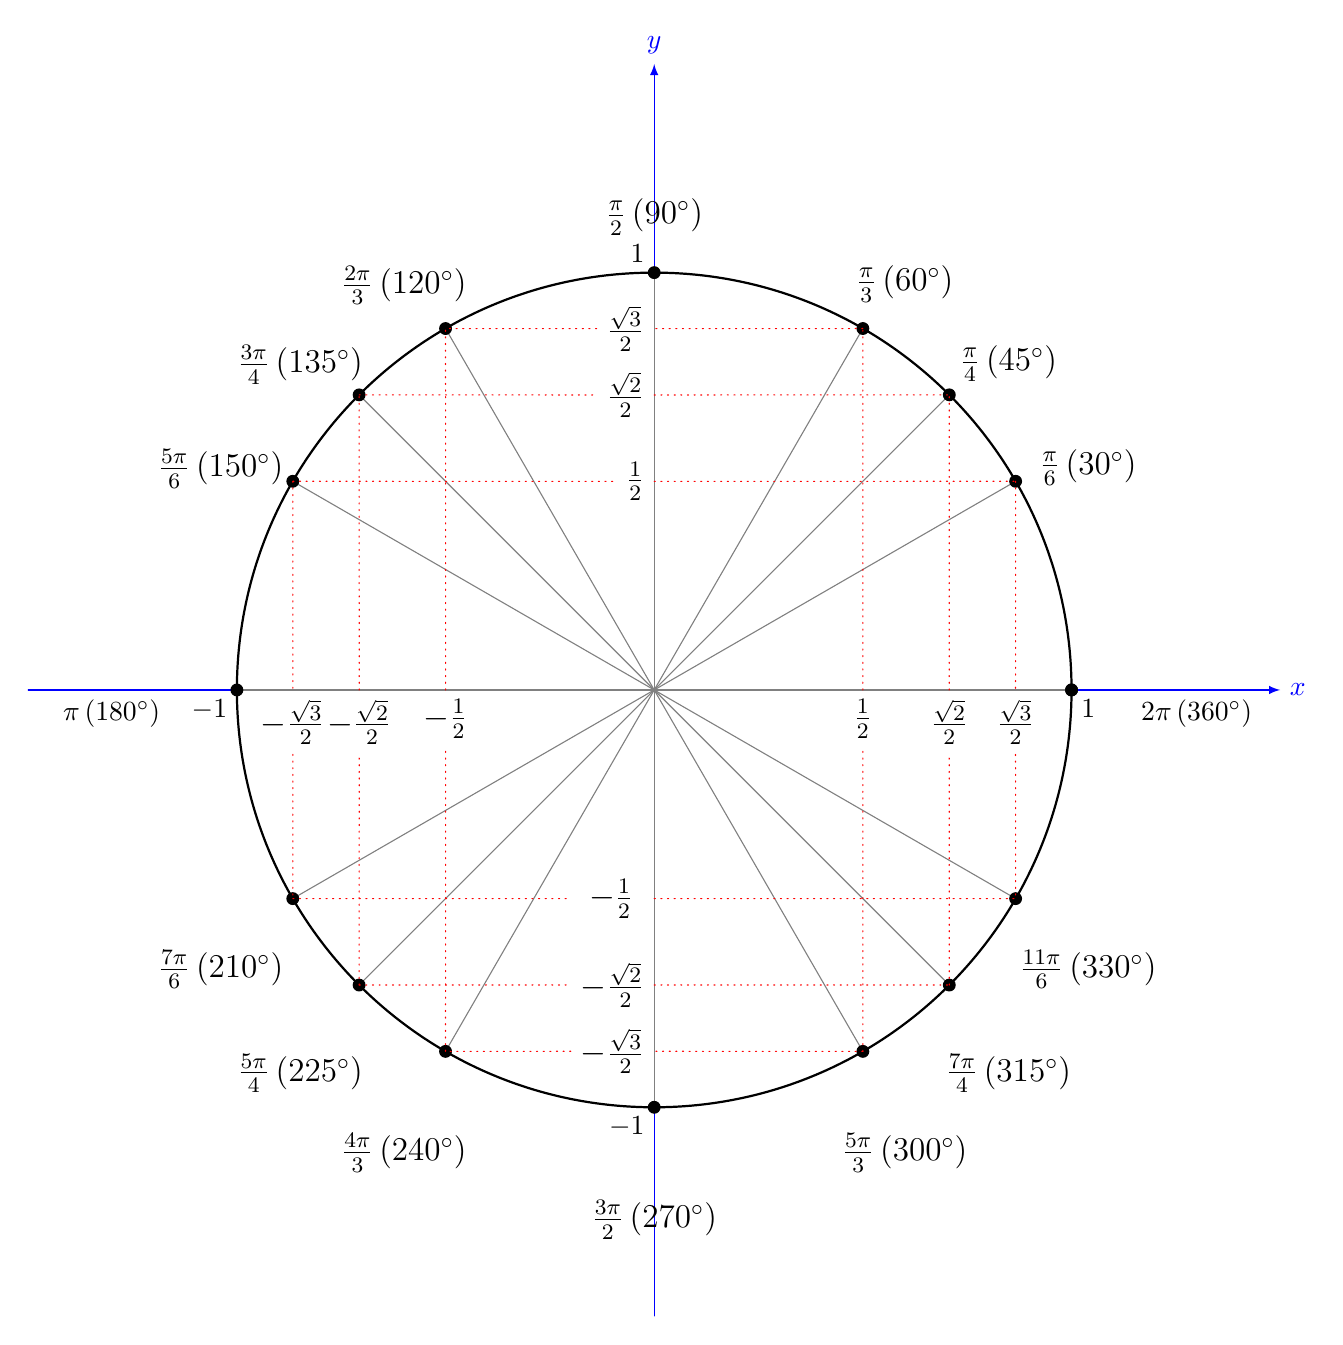
\begin{tikzpicture}[scale=5.3,cap=round,>=latex]

        % draw the coordinates
        \draw[->, color=blue] (-1.5cm,0cm) -- (1.5cm,0cm) node[right] {$x$};
        \draw[->, color=blue] (0cm,-1.5cm) -- (0cm,1.5cm) node[above,] {$y$};

        % draw the unit circle
        \draw[thick] (0cm,0cm) circle(1cm);

        \foreach \x in {0,30,...,360} {
                % lines from center to point
                \draw[gray] (0cm,0cm) -- (\x:1cm);
                % dots at each point
                \filldraw[black] (\x:1cm) circle(0.4pt);
                % draw each angle in degrees
                %\draw (\x:0.6cm) node[fill=white] {$\x^\circ$};
        }
        \foreach \n in {45, 135, 225, 315} {
        \draw[gray] (0cm,0cm) -- (\n:1cm);
        \filldraw[black] (\n:1cm) circle(0.4pt);
        }
        % draw each angle in radians
        \foreach \x/\xtext in {
            30/\frac{\pi}{6} \, (30^\circ),
            45/\frac{\pi}{4} \, (45^\circ),
            60/\frac{\pi}{3} \, (60^\circ),
            90/\frac{\pi}{2} \, (90^\circ),
            120/\frac{2\pi}{3} \, (120^\circ),
            135/\frac{3\pi}{4} \, (135^\circ),
            150/\frac{5\pi}{6} \, (150^\circ),
            %180/\pi \, (180^\circ),
            210/\frac{7\pi}{6} \, (210^\circ),
            225/\frac{5\pi}{4}\, (225^\circ),
            240/\frac{4\pi}{3}\, (240^\circ),
            270/\frac{3\pi}{2}\, (270^\circ),
            300/\frac{5\pi}{3} \, (300^\circ),
            315/\frac{7\pi}{4} \, (315^\circ),
            330/\frac{11\pi}{6} \, (330^\circ)
            %360/2\pi \, (360^\circ)
            }
                \draw (\x:1.2cm) node[anchor=north] {\large $\xtext$};

        \draw (180:1.3 cm) node[anchor=north] {$\pi \, (180^\circ)$};
        \draw (0:1.3 cm) node[anchor=north] {$2\pi \, (360^\circ)$};

        \node[anchor=north west] (xas) at (1,0) {$1$};
        \node[anchor=north east] (xas2) at (-1,0) {$-1$};
        \node[anchor=south east] (yas) at (0,1) {$1$};
        \node[anchor=north east] (yas2) at (0,-1) {$-1$};

        \node[anchor=east] (jy1) at (0,0.5) {\large $\frac12$};
        \node[anchor=east] (jy2) at (0,0.707) {\large $\frac{\sqrt{2}}{2}$};
        \node[anchor=east] (jy3) at (0,0.866) {\large $\frac{\sqrt{3}}{2}$};

        \draw[dotted, color=red]
        (-0.866,0.5)--(jy1)--(0.866,0.5)
        (-0.707,0.707)--(jy2)--(0.707,0.707)
        (0.5,0.866)--(jy3)--(-0.5,0.866)
        ;

        \node[anchor=north] (jx1) at (0.5,0) { \large $\frac12$};
        \node[anchor=north] (jx2) at (0.707,0) { \large $\frac{\sqrt{2}}{2}$};
        \node[anchor=north] (jx3) at (0.866,0) {\large $\frac{\sqrt{3}}{2}$};

        \draw[dotted, color=red]
        (0.5,-0.866)--(jx1)--(0.5,0.866)
        (0.707,-0.707)--(jx2)--(0.707,0.707)
        (0.866,0.5)--(jx3)--(0.866,-0.5)
        ;
        % draw the horizontal and vertical coordinates
        % the placement is better this way
        \node[shape=circle,anchor=east] (ny1) at (0,-0.5) { \large $-\frac12$};
        \node[anchor=east] (ny2) at (0,-0.707) {\large $-\frac{\sqrt{2}}{2}$};
        \node[anchor=east] (ny3) at (0,-0.866) {\large $-\frac{\sqrt{3}}{2}$};

        \draw[dotted, color=red]
        (-0.866,-0.5)--(ny1)--(0.866,-0.5)
        (-0.707,-0.707)--(ny2)--(0.707,-0.707)
        (0.5,-0.866)--(ny3)--(-0.5,-0.866)
        ;

        \node[anchor=north] (nx1) at (-0.5,0) {\large $-\frac12$};
        \node[anchor=north] (nx2) at (-0.707,0) {\large $-\frac{\sqrt{2}}{2}$};
        \node[anchor=north] (nx3) at (-0.866,0) {\large $-\frac{\sqrt{3}}{2}$};

        \draw[dotted, color=red]
        (-0.5,-0.866)--(nx1)--(-0.5,0.866)
        (-0.707,-0.707)--(nx2)--(-0.707,0.707)
        (-0.866,0.5)--(nx3)--(-0.866,-0.5)
        ;

    \end{tikzpicture}
\end{document}
